\documentclass[border=6pt]{standalone}
\usepackage{amsmath,amssymb}
\usepackage[dvipsnames]{xcolor}
\usepackage{tikz}
\definecolor{goodpurple}{HTML}{E771DF}
\definecolor{orange(ryb)}{HTML}{FFA500}
\definecolor{dodgerblue}{HTML}{1E90FF}
\colorlet{cz1color}{PineGreen}
\colorlet{cz2color}{LimeGreen}
\begin{document}
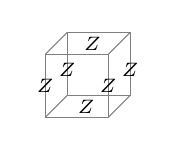
\begin{tikzpicture}[scale = 0.4, baseline={([yshift=-.5ex]current bounding box.center)}]
  % Define the vertices of the cube
  \coordinate (A) at (0, 0);
  \coordinate (B) at (2, 0);
  \coordinate (C) at (2, 2);
  \coordinate (D) at (0, 2);
  \coordinate (E) at (0.7, 0.7);
  \coordinate (F) at (2.7, 0.7);
  \coordinate (G) at (2.7, 2.7);
  \coordinate (H) at (0.7, 2.7);
  % Draw the back face
  \draw[color = gray] (E) -- (F) -- (G) -- (H) -- cycle;
  % Draw the front face
  \draw[color = gray] (A) -- (B) -- (C) -- (D) -- cycle;
  % Connect the corresponding vertices
  \draw[color = gray] (A) -- (E);
  \draw[color = gray] (B) -- (F);
  \draw[color = gray] (C) -- (G);
  \draw[color = gray] (D) -- (H);
  \node at (0, 1) {\scriptsize $Z$};
  \node at (0.7, 1.5) {\scriptsize $Z$};%^{\dagger}$};
  \node at (2, 1) {\scriptsize $Z$};%^{\dagger}$};
  \node at (2.7, 1.5) {\scriptsize $Z$};
  \node at (1.3, 0.35) {\scriptsize $Z$};
  \node at (1.5, 0.35 + 2) {\scriptsize $Z$};%^{\dagger}$};
\end{tikzpicture}
\hspace{16pt}
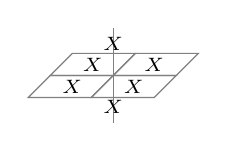
\begin{tikzpicture}[scale = 0.4, baseline={([yshift=-.5ex]current bounding box.center)}]
    \coordinate (A) at (0, 0);
    \coordinate (Azp) at (0, 1.5); % 2 
    \coordinate (Azm) at (0, -1.5); %2
    \coordinate (B) at (0.7, 0.7);
    \coordinate (C) at (2.7, 0.7);
    \coordinate (D) at (2, 0);
    \coordinate (E) at (-0.7, -0.7);
    \coordinate (F) at (-2.7, -0.7);
    \coordinate (G) at (-2, 0);
    \coordinate (H) at (-1.3, 0.7);
    \coordinate (I) at (1.3, -0.7);
    %
    \draw[color = gray] (A) -- (B) -- (C) -- (D)--cycle;
    \draw[color = gray] (A) -- (E) -- (F) -- (G)--cycle;
    \draw[color = gray] (A) -- (B) -- (H) -- (G)--cycle;
    \draw[color = gray] (A) -- (E) -- (I) -- (D)--cycle;
    \draw[color = gray] (Azm) -- (Azp);

    \node at (-2.6/2, -0.7/2) {\scriptsize $X$}; % F/2
    \node at (2.6/2, 0.7/2) {\scriptsize $X$};
    \node at (-1.3/2, 0.7/2) {\scriptsize $X$};%^{\dagger}$}; % H/2
    \node at (1.3/2, -0.7/2) {\scriptsize $X$};%^{\dagger}$}; % H/2
    \node at (0, 1.) {\scriptsize $X$};%^{\dagger}$};
    \node at (0, -1.) {\scriptsize $X$};
\end{tikzpicture}
\end{document}
